\documentclass[]{article}
\usepackage{lmodern}
\usepackage{amssymb,amsmath}
\usepackage{ifxetex,ifluatex}
\usepackage{fixltx2e} % provides \textsubscript
\ifnum 0\ifxetex 1\fi\ifluatex 1\fi=0 % if pdftex
  \usepackage[T1]{fontenc}
  \usepackage[utf8]{inputenc}
\else % if luatex or xelatex
  \ifxetex
    \usepackage{mathspec}
    \usepackage{xltxtra,xunicode}
  \else
    \usepackage{fontspec}
  \fi
  \defaultfontfeatures{Mapping=tex-text,Scale=MatchLowercase}
  \newcommand{\euro}{€}
\fi
% use upquote if available, for straight quotes in verbatim environments
\IfFileExists{upquote.sty}{\usepackage{upquote}}{}
% use microtype if available
\IfFileExists{microtype.sty}{%
\usepackage{microtype}
\UseMicrotypeSet[protrusion]{basicmath} % disable protrusion for tt fonts
}{}
\usepackage[margin=1in]{geometry}
\usepackage{color}
\usepackage{fancyvrb}
\newcommand{\VerbBar}{|}
\newcommand{\VERB}{\Verb[commandchars=\\\{\}]}
\DefineVerbatimEnvironment{Highlighting}{Verbatim}{commandchars=\\\{\}}
% Add ',fontsize=\small' for more characters per line
\usepackage{framed}
\definecolor{shadecolor}{RGB}{248,248,248}
\newenvironment{Shaded}{\begin{snugshade}}{\end{snugshade}}
\newcommand{\KeywordTok}[1]{\textcolor[rgb]{0.13,0.29,0.53}{\textbf{{#1}}}}
\newcommand{\DataTypeTok}[1]{\textcolor[rgb]{0.13,0.29,0.53}{{#1}}}
\newcommand{\DecValTok}[1]{\textcolor[rgb]{0.00,0.00,0.81}{{#1}}}
\newcommand{\BaseNTok}[1]{\textcolor[rgb]{0.00,0.00,0.81}{{#1}}}
\newcommand{\FloatTok}[1]{\textcolor[rgb]{0.00,0.00,0.81}{{#1}}}
\newcommand{\CharTok}[1]{\textcolor[rgb]{0.31,0.60,0.02}{{#1}}}
\newcommand{\StringTok}[1]{\textcolor[rgb]{0.31,0.60,0.02}{{#1}}}
\newcommand{\CommentTok}[1]{\textcolor[rgb]{0.56,0.35,0.01}{\textit{{#1}}}}
\newcommand{\OtherTok}[1]{\textcolor[rgb]{0.56,0.35,0.01}{{#1}}}
\newcommand{\AlertTok}[1]{\textcolor[rgb]{0.94,0.16,0.16}{{#1}}}
\newcommand{\FunctionTok}[1]{\textcolor[rgb]{0.00,0.00,0.00}{{#1}}}
\newcommand{\RegionMarkerTok}[1]{{#1}}
\newcommand{\ErrorTok}[1]{\textbf{{#1}}}
\newcommand{\NormalTok}[1]{{#1}}
\usepackage{longtable,booktabs}
\usepackage{graphicx}
\makeatletter
\def\maxwidth{\ifdim\Gin@nat@width>\linewidth\linewidth\else\Gin@nat@width\fi}
\def\maxheight{\ifdim\Gin@nat@height>\textheight\textheight\else\Gin@nat@height\fi}
\makeatother
% Scale images if necessary, so that they will not overflow the page
% margins by default, and it is still possible to overwrite the defaults
% using explicit options in \includegraphics[width, height, ...]{}
\setkeys{Gin}{width=\maxwidth,height=\maxheight,keepaspectratio}
\ifxetex
  \usepackage[setpagesize=false, % page size defined by xetex
              unicode=false, % unicode breaks when used with xetex
              xetex]{hyperref}
\else
  \usepackage[unicode=true]{hyperref}
\fi
\hypersetup{breaklinks=true,
            bookmarks=true,
            pdfauthor={Daniel Brooks (daniel.brooks@spsmail.cuny.edu), Daniel Fanelli (daniel.fanelli@spsmail.cuny.edu), Christopher Fenton (christopher.fenton@spsmail.cuny.edu), James Hamski (james.hamski@spsmail.cuny.edu), Youqing Xiang (youqing.xiang@spsmail.cuny.edu)},
            pdftitle={Predicting Car Crash and Cost data From Insurance Data},
            colorlinks=true,
            citecolor=blue,
            urlcolor=blue,
            linkcolor=magenta,
            pdfborder={0 0 0}}
\urlstyle{same}  % don't use monospace font for urls
\setlength{\parindent}{0pt}
\setlength{\parskip}{6pt plus 2pt minus 1pt}
\setlength{\emergencystretch}{3em}  % prevent overfull lines
\setcounter{secnumdepth}{5}

%%% Use protect on footnotes to avoid problems with footnotes in titles
\let\rmarkdownfootnote\footnote%
\def\footnote{\protect\rmarkdownfootnote}

%%% Change title format to be more compact
\usepackage{titling}

% Create subtitle command for use in maketitle
\newcommand{\subtitle}[1]{
  \posttitle{
    \begin{center}\large#1\end{center}
    }
}

\setlength{\droptitle}{-2em}
  \title{Predicting Car Crash and Cost data From Insurance Data}
  \pretitle{\vspace{\droptitle}\centering\huge}
  \posttitle{\par}
  \author{Daniel Brooks
(\href{mailto:daniel.brooks@spsmail.cuny.edu}{\nolinkurl{daniel.brooks@spsmail.cuny.edu}}),
Daniel Fanelli
(\href{mailto:daniel.fanelli@spsmail.cuny.edu}{\nolinkurl{daniel.fanelli@spsmail.cuny.edu}}),
Christopher Fenton
(\href{mailto:christopher.fenton@spsmail.cuny.edu}{\nolinkurl{christopher.fenton@spsmail.cuny.edu}}),
James Hamski
(\href{mailto:james.hamski@spsmail.cuny.edu}{\nolinkurl{james.hamski@spsmail.cuny.edu}}),
Youqing Xiang
(\href{mailto:youqing.xiang@spsmail.cuny.edu}{\nolinkurl{youqing.xiang@spsmail.cuny.edu}})}
  \preauthor{\centering\large\emph}
  \postauthor{\par}
  \predate{\centering\large\emph}
  \postdate{\par}
  \date{7/10/2016}



\begin{document}

\maketitle


\section{Introduction}\label{introduction}

The purpose of this assignment is to build a series two different
models. The first model will predict whether a person will get into a
car crash and the second model will be used to predict the amount as to
which the crash will cost. Both of these models will utilize the
customers insurnace information to predict the two variables stated
above.

Our data consists of 8161 customers with 24 potential predictor
variables and 2 target (response) variables. The response variables are:

TARGET\_FLAG: This flag will take a value of 0 or 1. One means that the
person was in a car crash and 0 means that they were not.

TARGET\_AMT: This is the amount associated with the car crash. If the
TARGET\_FLAG field is 0, then there will be no amount, because the
person did not get into a crash. If the TARGET\_FLAG is a 1, then there
will be a value in this field, because there was a crash.

\section{Data Exploration}\label{data-exploration}

The first thing that has to be taken care of is the missing (NA) values
in the data. We can see that in Figure 1.1, there are a few fields that
have some missing values. We can see that the fields JOB, CAR\_AGE,
HOME\_VAL, YOJ, AGE and INCOME have missing values. These need to either
be removed or imputed to continue on with the analysis.

Figure 1.1
\includegraphics{DATA621-Homework-4_files/figure-latex/unnamed-chunk-3-1.pdf}

We can also see, in the summary statistics (Figure 1.2) some of the data
is incorrect. The CAR\_AGE filed is showing that the minimum car age is
-3. That is not a possible value for that field. That field will have to
be looked at more closely to see what other values are invalid. They
will have to be re-imputed or removed before the final models are
created.

The data also contains 10 categorical variables and 16 numeric
variables. The categorical data will need to be converted into a
numerical field in order to be plugged into the model and get a value
for the two target variables.

Figure 1.2

\begin{verbatim}
##      INDEX        TARGET_FLAG       TARGET_AMT        KIDSDRIV     
##  Min.   :    1   Min.   :0.0000   Min.   :     0   Min.   :0.0000  
##  1st Qu.: 2559   1st Qu.:0.0000   1st Qu.:     0   1st Qu.:0.0000  
##  Median : 5133   Median :0.0000   Median :     0   Median :0.0000  
##  Mean   : 5152   Mean   :0.2638   Mean   :  1504   Mean   :0.1711  
##  3rd Qu.: 7745   3rd Qu.:1.0000   3rd Qu.:  1036   3rd Qu.:0.0000  
##  Max.   :10302   Max.   :1.0000   Max.   :107586   Max.   :4.0000  
##                                                                    
##       AGE           HOMEKIDS           YOJ          INCOME         
##  Min.   :16.00   Min.   :0.0000   Min.   : 0.0   Length:8161       
##  1st Qu.:39.00   1st Qu.:0.0000   1st Qu.: 9.0   Class :character  
##  Median :45.00   Median :0.0000   Median :11.0   Mode  :character  
##  Mean   :44.79   Mean   :0.7212   Mean   :10.5                     
##  3rd Qu.:51.00   3rd Qu.:1.0000   3rd Qu.:13.0                     
##  Max.   :81.00   Max.   :5.0000   Max.   :23.0                     
##  NA's   :6                        NA's   :454                      
##    PARENT1            HOME_VAL           MSTATUS         
##  Length:8161        Length:8161        Length:8161       
##  Class :character   Class :character   Class :character  
##  Mode  :character   Mode  :character   Mode  :character  
##                                                          
##                                                          
##                                                          
##                                                          
##      SEX             EDUCATION             JOB               TRAVTIME     
##  Length:8161        Length:8161        Length:8161        Min.   :  5.00  
##  Class :character   Class :character   Class :character   1st Qu.: 22.00  
##  Mode  :character   Mode  :character   Mode  :character   Median : 33.00  
##                                                           Mean   : 33.49  
##                                                           3rd Qu.: 44.00  
##                                                           Max.   :142.00  
##                                                                           
##    CAR_USE            BLUEBOOK              TIF           CAR_TYPE        
##  Length:8161        Length:8161        Min.   : 1.000   Length:8161       
##  Class :character   Class :character   1st Qu.: 1.000   Class :character  
##  Mode  :character   Mode  :character   Median : 4.000   Mode  :character  
##                                        Mean   : 5.351                     
##                                        3rd Qu.: 7.000                     
##                                        Max.   :25.000                     
##                                                                           
##    RED_CAR            OLDCLAIM            CLM_FREQ        REVOKED         
##  Length:8161        Length:8161        Min.   :0.0000   Length:8161       
##  Class :character   Class :character   1st Qu.:0.0000   Class :character  
##  Mode  :character   Mode  :character   Median :0.0000   Mode  :character  
##                                        Mean   :0.7986                     
##                                        3rd Qu.:2.0000                     
##                                        Max.   :5.0000                     
##                                                                           
##     MVR_PTS          CAR_AGE        URBANICITY       
##  Min.   : 0.000   Min.   :-3.000   Length:8161       
##  1st Qu.: 0.000   1st Qu.: 1.000   Class :character  
##  Median : 1.000   Median : 8.000   Mode  :character  
##  Mean   : 1.696   Mean   : 8.328                     
##  3rd Qu.: 3.000   3rd Qu.:12.000                     
##  Max.   :13.000   Max.   :28.000                     
##                   NA's   :510
\end{verbatim}

In Figure 1.3 we take a look at the first target variable
(TARGET\_FLAG). The summary stats are saying that the mean is less than
.5 which means that the data is not evenly disbursd between 0 and 1. The
mean would be .5 if that were the case. We can see by the histogram that
there are about 3 times as many 0's (no crashes) then there are crashes
in this data set. In Figure 1.4, we see that the amount that the
customer paid is also around 0. That is agreeing with the high amount of
no crashes that we saw in Figure 1.3. This means we can procede with our
analysis.

Figure 1.3

\begin{verbatim}
##    Min. 1st Qu.  Median    Mean 3rd Qu.    Max. 
##  0.0000  0.0000  0.0000  0.2638  1.0000  1.0000
\end{verbatim}

\includegraphics{DATA621-Homework-4_files/figure-latex/unnamed-chunk-5-1.pdf}

Figure 1.3

\begin{verbatim}
##    Min. 1st Qu.  Median    Mean 3rd Qu.    Max. 
##       0       0       0    1504    1036  107600
\end{verbatim}

\includegraphics{DATA621-Homework-4_files/figure-latex/unnamed-chunk-6-1.pdf}

Finally, we want to look at the variables and see how they correlate
with each other. In Figure 1.5 we see a grid that plots each field in
the data set against each other. It also shows how strong of a
correlation there is between each variable through the correlation value
and the amount of starts in each box (correlation significance), 3
starts means that the variables have a very strong correlation and the
strength drops as the number of starts drop.

We can see from the grid, that not all of the variables correlate with
each other. The variables that appear to not make good predictors would
be, MVR\_PTS, TRAVTIME, and TIF. These variables have a loew correlation
signifiance. This means that they may not be good choices to include in
out final model for any of the target variables. All of the other
variables appear to have a relatively strong correlation between each
other and would be good choices for the overall model.

Figure 1.5
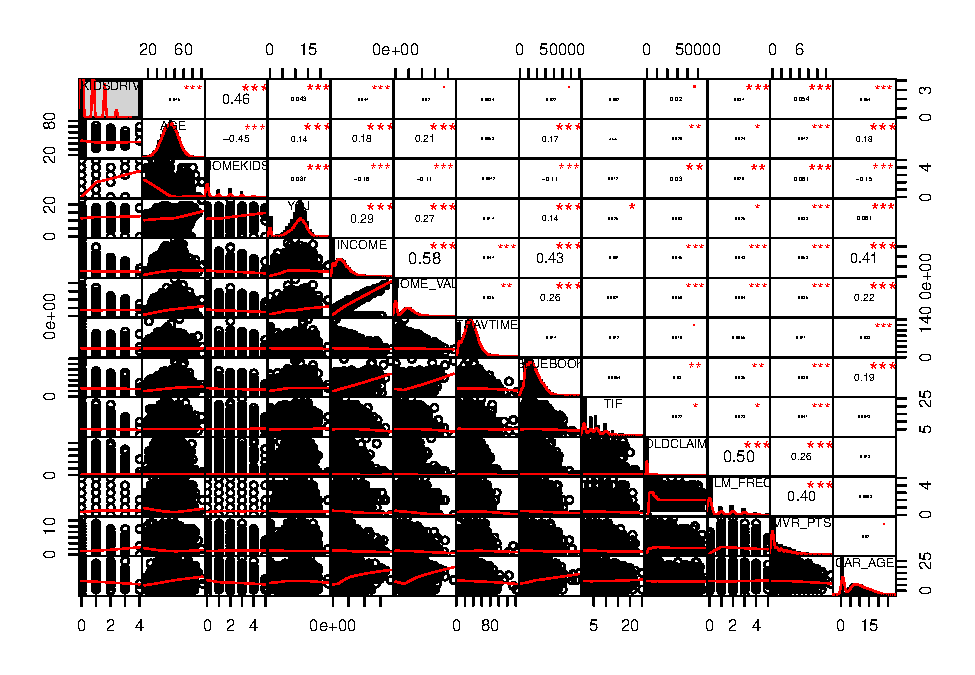
\includegraphics{DATA621-Homework-4_files/figure-latex/unnamed-chunk-7-1.pdf}

Firgue 1.6 is another way to show the correlation between variables,
just like in Figure 1.5. This grid has different color/size circles
within each variable intersection in the grid. The bigger the circle the
better the correlation. We can see that the fields TIF, TRAVTIME, and
MVR\_PTS are still relatively bad choices for variables, just like in
Figure 1.5.

Figure 1.6
\includegraphics{DATA621-Homework-4_files/figure-latex/unnamed-chunk-8-1.pdf}

\section{Data Preparation}\label{data-preparation}

\subsection{Dealing with NA's and Invalid
Values}\label{dealing-with-nas-and-invalid-values}

The first thing that we want to take care of is the NA's (missing
values) in the data. We decided that the best course of action would be
to remove any of the records that were not complete. Also, we will
remove any of the data that is invalid (like a car age below 0). With
the removal of the NA's and the invalid values, the total observations
for the data is reduced from 8161 to 6044 total obsverations. That is
still plenty of observations to do analysis and modeling on.

\subsection{Categorical Data}\label{categorical-data}

Within our data, there are 10 fields that are categorical. These
variables group the data into different sections. The best way to deal
with this data is to make dummy variables. Most of the data contains 1
of 2 posibilities (YES/NO etc). This allows me to assign a value of 0
for one possibility and a 1 for another. It changes the factor data into
a number so it can be used in the regression analysis. The education and
jobs fields were a little different. They have more than 2
possibilities. I grouped the possibilities intoe logical groups. The
eductaion was grouped by level of academic achievement (Masters and
above = 1, below is a 0). The education was grouped along the same way,
a college education/advanced education was grouped into on (Lwyer,
Professional, Manager = 1), everybody else gets a 0. The field of
CAR\_TYPE is dealt the same way as well. Those who drive a Panel Truck,
Pickup or Sports car will be labeled with a 1 and everything else will
be labeled with a 0.

\subsection{Accounting Type Data}\label{accounting-type-data}

The last thing that needed to be done with the data is to convert the
accouting data, into numeric fields. The accounting data (dollar amount
data) has dollar signs within the data. That means that the data will be
treated as a character set. The dollar sign needs to be removed and the
data needs to be changed into a number, so it can be used in the
analysis later on.

\section{Build Models}\label{build-models}

\subsection{TARGET\_FLAG}\label{targetux5fflag}

This is the target variable that will tell us there was a crash or not
for the given customer. If the field takes a value of 0, that means that
the customer was not in an accident, or the accident was not their
fault. If the field takes a value of 1, that means the customer has been
in an accident, or the accident was their fault.

The first thing that we need to do is split the data up into a training
set and a test set. We will be taking the data and separating it up so
70\% of the data is the training set, and 30\% of the data will be the
testing set.

\subsubsection{Model 1}\label{model-1}

In this model we are doing a type of stepwise function. We are taking
the training set and removing some of the variables that we feel are not
good predictors. We run the model against the remaining variables and
look at the output. Then, we go back through and remove anymore
variables that we do not feel are good predictors. That will leave us
with a final function that has all the variables that we fell will make
the best predicting function.

The output for this function is as follows:

\begin{verbatim}
## 
## Call:
## lm(formula = TARGET_FLAG ~ TARGET_AMT + PARENT1 + HOME_VAL + 
##     MSTATUS + TRAVTIME + CAR_USE + REVOKED + CAR_AGE + URBANICITY, 
##     data = training_2a)
## 
## Residuals:
##     Min      1Q  Median      3Q     Max 
## -3.2636 -0.2233 -0.1122  0.1505  1.0323 
## 
## Coefficients:
##               Estimate Std. Error t value Pr(>|t|)    
## (Intercept)  1.991e-01  2.728e-02   7.300 3.42e-13 ***
## TARGET_AMT   4.619e-05  1.205e-06  38.342  < 2e-16 ***
## PARENT1     -9.672e-02  1.775e-02  -5.450 5.34e-08 ***
## HOME_VAL    -4.393e-07  5.134e-08  -8.557  < 2e-16 ***
## MSTATUS     -6.171e-03  1.383e-02  -0.446    0.656    
## TRAVTIME     1.896e-03  3.404e-04   5.569 2.73e-08 ***
## CAR_USE     -1.009e-01  1.153e-02  -8.755  < 2e-16 ***
## REVOKED      1.125e-01  1.630e-02   6.904 5.81e-12 ***
## CAR_AGE     -4.603e-03  1.008e-03  -4.565 5.13e-06 ***
## URBANICITY   2.217e-01  1.356e-02  16.349  < 2e-16 ***
## ---
## Signif. codes:  0 '***' 0.001 '**' 0.01 '*' 0.05 '.' 0.1 ' ' 1
## 
## Residual standard error: 0.3476 on 4221 degrees of freedom
## Multiple R-squared:  0.3816, Adjusted R-squared:  0.3803 
## F-statistic: 289.4 on 9 and 4221 DF,  p-value: < 2.2e-16
\end{verbatim}

\subsubsection{Model 2}\label{model-2}

In this model, we are untilizing a backwards approach into solving for
the overall model. The backwards approach to variable selection starts
off withh all variables in the model. I then starts to remove fields,
until it gets to a point where removing anymore fields will not be
beneficial to the model. That is the point when the final model is
found.

To solve for the TARGET\_FLAG field, I will be using a probit function.
This function is very useful when there are only two possible outcomes
for the field that you are trying to predict. This model utilizes
backwards selection when picking the variables for the model. It starts
out all of the variables that are possible. It then starts to remove
variables until it reaches the optimal solution for the function. The
output from the model is as follows:

\begin{verbatim}
## 
## Call:
## glm(formula = TARGET_FLAG ~ KIDSDRIV + HOMEKIDS + INCOME + PARENT1 + 
##     HOME_VAL + MSTATUS + JOB + TRAVTIME + CAR_USE + BLUEBOOK + 
##     TIF + CAR_TYPE + RED_CAR + OLDCLAIM + CLM_FREQ + REVOKED + 
##     MVR_PTS + CAR_AGE + URBANICITY, family = binomial(link = "probit"), 
##     data = train1)
## 
## Deviance Residuals: 
##     Min       1Q   Median       3Q      Max  
## -2.4940  -0.7389  -0.4044   0.6440   3.0326  
## 
## Coefficients:
##               Estimate Std. Error z value Pr(>|z|)    
## (Intercept) -1.195e+00  1.606e-01  -7.443 9.88e-14 ***
## KIDSDRIV     1.687e-01  4.850e-02   3.479 0.000503 ***
## HOMEKIDS     5.036e-02  2.728e-02   1.846 0.064869 .  
## INCOME      -2.217e-06  7.921e-07  -2.799 0.005121 ** 
## PARENT1     -1.895e-01  8.692e-02  -2.181 0.029213 *  
## HOME_VAL    -9.539e-07  2.847e-07  -3.350 0.000809 ***
## MSTATUS      2.626e-01  6.829e-02   3.846 0.000120 ***
## JOB         -1.446e-01  5.068e-02  -2.852 0.004340 ** 
## TRAVTIME     9.112e-03  1.482e-03   6.147 7.91e-10 ***
## CAR_USE     -4.762e-01  5.247e-02  -9.075  < 2e-16 ***
## BLUEBOOK    -1.499e-05  3.213e-06  -4.666 3.07e-06 ***
## TIF         -3.352e-02  5.830e-03  -5.749 8.96e-09 ***
## CAR_TYPE     2.303e-01  5.001e-02   4.605 4.12e-06 ***
## RED_CAR     -2.417e-01  5.374e-02  -4.498 6.87e-06 ***
## OLDCLAIM    -9.334e-06  3.273e-06  -2.852 0.004345 ** 
## CLM_FREQ     1.645e-01  2.286e-02   7.197 6.17e-13 ***
## REVOKED      5.153e-01  7.461e-02   6.906 4.98e-12 ***
## MVR_PTS      6.924e-02  1.105e-02   6.269 3.63e-10 ***
## CAR_AGE     -1.175e-02  4.772e-03  -2.462 0.013818 *  
## URBANICITY   1.195e+00  7.684e-02  15.549  < 2e-16 ***
## ---
## Signif. codes:  0 '***' 0.001 '**' 0.01 '*' 0.05 '.' 0.1 ' ' 1
## 
## (Dispersion parameter for binomial family taken to be 1)
## 
##     Null deviance: 4896.6  on 4230  degrees of freedom
## Residual deviance: 3817.2  on 4211  degrees of freedom
## AIC: 3857.2
## 
## Number of Fisher Scoring iterations: 5
\end{verbatim}

\subsubsection{Model 3}\label{model-3}

The model is a little interesting in the fact that, the original
analysis of the data showed that the fields TIF, TRAVTIME and MVR\_PTS
were not good predictors. They all had very few starts when being
correlated with the other variables. They all showed up in the model.
This could be due to the fact that the original analysis was based on a
linear comparision. This equation is a log function. That shows that
those variables may have a horrible linear relationship with the rest of
the variables but a very stong logistic relationship.

To solve for the TARGET\_FLAG field, I will be using a probit function,
just like during the backwards function. This function goes the opposite
way as the backward function. It starts with a plain function and adds
variables until it gets to the optimal solution. Once it cannot add
variables to make the equation better, it stops and that is the final
function. The output for the forward stepping function is as follows:

\begin{verbatim}
## 
## Call:
## glm(formula = TARGET_FLAG ~ URBANICITY + HOME_VAL + CLM_FREQ + 
##     CAR_USE + MVR_PTS + REVOKED + PARENT1 + TRAVTIME + BLUEBOOK + 
##     TIF + RED_CAR + CAR_AGE + CAR_TYPE + KIDSDRIV + JOB + OLDCLAIM + 
##     MSTATUS + INCOME + HOMEKIDS, family = binomial(link = "probit"), 
##     data = train1)
## 
## Deviance Residuals: 
##     Min       1Q   Median       3Q      Max  
## -2.4940  -0.7389  -0.4044   0.6440   3.0326  
## 
## Coefficients:
##               Estimate Std. Error z value Pr(>|z|)    
## (Intercept) -1.195e+00  1.606e-01  -7.443 9.88e-14 ***
## URBANICITY   1.195e+00  7.684e-02  15.549  < 2e-16 ***
## HOME_VAL    -9.539e-07  2.847e-07  -3.350 0.000809 ***
## CLM_FREQ     1.645e-01  2.286e-02   7.197 6.17e-13 ***
## CAR_USE     -4.762e-01  5.247e-02  -9.075  < 2e-16 ***
## MVR_PTS      6.924e-02  1.105e-02   6.269 3.63e-10 ***
## REVOKED      5.153e-01  7.461e-02   6.906 4.98e-12 ***
## PARENT1     -1.895e-01  8.692e-02  -2.181 0.029213 *  
## TRAVTIME     9.112e-03  1.482e-03   6.147 7.91e-10 ***
## BLUEBOOK    -1.499e-05  3.213e-06  -4.666 3.07e-06 ***
## TIF         -3.352e-02  5.830e-03  -5.749 8.96e-09 ***
## RED_CAR     -2.417e-01  5.374e-02  -4.498 6.87e-06 ***
## CAR_AGE     -1.175e-02  4.772e-03  -2.462 0.013818 *  
## CAR_TYPE     2.303e-01  5.001e-02   4.605 4.12e-06 ***
## KIDSDRIV     1.687e-01  4.850e-02   3.479 0.000503 ***
## JOB         -1.446e-01  5.068e-02  -2.852 0.004340 ** 
## OLDCLAIM    -9.334e-06  3.273e-06  -2.852 0.004345 ** 
## MSTATUS      2.626e-01  6.829e-02   3.846 0.000120 ***
## INCOME      -2.217e-06  7.921e-07  -2.799 0.005121 ** 
## HOMEKIDS     5.036e-02  2.728e-02   1.846 0.064869 .  
## ---
## Signif. codes:  0 '***' 0.001 '**' 0.01 '*' 0.05 '.' 0.1 ' ' 1
## 
## (Dispersion parameter for binomial family taken to be 1)
## 
##     Null deviance: 4896.6  on 4230  degrees of freedom
## Residual deviance: 3817.2  on 4211  degrees of freedom
## AIC: 3857.2
## 
## Number of Fisher Scoring iterations: 5
\end{verbatim}

This functions is very interesting. In the backwards function, stated
above (Model 1), the MSTATUS (Marital status) field is positive, but it
is negative in the forwards function. The sign swtiched depending on
which way ypu come at the optimal function. Since the model also
contains the field of KIDSDRIV and PARENT1, it is possible that
multicolinearity could be playing a factor. It is also very interesting
that the TRAVTIME, TIF and MVR\_PTS fields are also included in this
model just like in the backwards model.

\subsubsection{Model 4 (Remove Redundancy, Calculate All
Combinations)}\label{model-4-remove-redundancy-calculate-all-combinations}

Because the data contains such a large number of categorical fields, it
is impossible (with our machine power + time constraints) to calculate
and test the model for all possible combinations of the categorical's
inclusion and/or values. However, what if some of the fields could
\textbf{\emph{simply be removed}}? Let's take a look at the
\textbf{\emph{correlations}} between some of the dependent attributes in
our data.

\begin{longtable}[c]{@{}lr@{}}
\toprule
col\_names & accuracy\tabularnewline
\midrule
\endhead
CAR\_TYPE & 0.7345154\tabularnewline
CAR\_USE & 0.7345154\tabularnewline
EDUCATION & 0.7345154\tabularnewline
JOB & 0.7345154\tabularnewline
MSTATUS & 0.7345154\tabularnewline
PARENT1 & 0.7345154\tabularnewline
RED\_CAR & 0.7345154\tabularnewline
REVOKED & 0.7345154\tabularnewline
SEX & 0.7345154\tabularnewline
URBANICITY & 0.7345154\tabularnewline
\bottomrule
\end{longtable}

\textbf{\emph{Those categorical variables have the exact same calculated
accuracties.}}

Could this be coincidence? Seems those columns could be duplicates,
let's run Chi-Square correlation tests to confirm:

\begin{longtable}[c]{@{}lr@{}}
\toprule
all\_chi\_sq\_labels & all\_chi\_sq\_results\tabularnewline
\midrule
\endhead
car\_type\_to\_car\_use & 0.000\tabularnewline
car\_type\_to\_education & 0.000\tabularnewline
car\_type\_to\_job & 0.366\tabularnewline
car\_type\_to\_mstatus & 0.229\tabularnewline
car\_type\_to\_parent1 & 0.630\tabularnewline
car\_type\_to\_red\_car & 0.000\tabularnewline
car\_type\_to\_revoked & 0.796\tabularnewline
car\_type\_to\_sex & 0.000\tabularnewline
car\_type\_to\_urbancity & 0.506\tabularnewline
\bottomrule
\end{longtable}

\textbf{\emph{Chi-Squared says some columns are exact duplicates: Remove
Them! (We'll keep CARTYPE):}}

Why can we simply remove fields? Imagine there is a categorical called
letters with ``a'',``b'',``c'',``d'' values. And there is a categorical
called numbers with ``one'',``two'',``three'',``four''. If for EVERY
occurence:

``a'' =\textgreater{} ``one'' ``b'' =\textgreater{} ``two'' ``c''
=\textgreater{} ``three'' ``d'' =\textgreater{} ``four''

Then would it make sense to calculate a model for all 16
letter-to-number commbinations? Of course not, they are 100\%
correlated. We can just keep one of the fields.

Also, \textbf{\emph{car\_type\_to\_mstatus}} and
\textbf{\emph{car\_type\_to\_revoked}} were close, lets compare mstatus
to revoked:

\begin{verbatim}
## [1] 0.002
\end{verbatim}

So those are ALSO \textbf{\emph{DUPLICATES}}, remove REVOKED

\begin{Shaded}
\begin{Highlighting}[]
\NormalTok{drops <-}\StringTok{ }\KeywordTok{c}\NormalTok{(}\StringTok{"REVOKED"}\NormalTok{)}
\NormalTok{ins.train <-}\StringTok{ }\NormalTok{ins.train[ , !(}\KeywordTok{names}\NormalTok{(ins.train) %in%}\StringTok{ }\NormalTok{drops)]}
\NormalTok{ins.test <-}\StringTok{ }\NormalTok{ins.test[ , !(}\KeywordTok{names}\NormalTok{(ins.test) %in%}\StringTok{ }\NormalTok{drops)]}
\end{Highlighting}
\end{Shaded}

So now that we have lowered our number of categorical variables, and
thus lowered the total number of possible categorical combinations to
calculate, we can use a tool ``grind out'' every combination and
evaluate based on whatever criteria we wish:

\textbf{\emph{Try out all categorical combinations with a tools, in this
case - MuMIn DREDGE}}

\begin{verbatim}
## Fixed term is "(Intercept)"
\end{verbatim}

\begin{longtable}[c]{@{}lrrrrrrrrrrrrrrrrrrrrrrr@{}}
\toprule
& (Intercept) & AGE & BLUEBOOK & CAR\_AGE & CAR\_TYPE & CLM\_FREQ &
HOME\_VAL & HOMEKIDS & INCOME & KIDSDRIV & MSTATUS & MVR\_PTS & OLDCLAIM
& TIF & TRAVTIME & YOJ & R\^{}2 & adjR\^{}2 & df & logLik & AIC & delta
& weight\tabularnewline
\midrule
\endhead
14208 & 0.2537193 & -0.0012133 & -2.3e-06 & -0.0043540 & 0.0829113 &
0.0648146 & -3e-07 & 0.0191497 & NA & 0.0446246 & 0.0751249 & 0.0268602
& NA & -0.0083465 & 0.0013801 & NA & 0.1431265 & 0.2045400 & 14 &
-2217.936 & 4463.872 & 0.0000000 & 0.2731834\tabularnewline
14207 & 0.2003112 & NA & -2.4e-06 & -0.0045619 & 0.0829143 & 0.0645957 &
-3e-07 & 0.0237367 & NA & 0.0414338 & 0.0765694 & 0.0270047 & NA &
-0.0083609 & 0.0013773 & NA & 0.1426986 & 0.2039285 & 13 & -2218.992 &
4463.983 & 0.1118193 & 0.2583289\tabularnewline
30591 & 0.2185462 & NA & -2.3e-06 & -0.0045474 & 0.0824832 & 0.0645880 &
-3e-07 & 0.0248347 & NA & 0.0412784 & 0.0763650 & 0.0269845 & NA &
-0.0082758 & 0.0013776 & -0.0022657 & 0.1431034 & 0.2045070 & 14 &
-2217.993 & 4463.986 & 0.1140088 & 0.2580463\tabularnewline
30592 & 0.2630198 & -0.0010646 & -2.2e-06 & -0.0043669 & 0.0825370 &
0.0647811 & -3e-07 & 0.0206664 & NA & 0.0440983 & 0.0751244 & 0.0268603
& NA & -0.0082744 & 0.0013801 & -0.0019693 & 0.1434259 & 0.2049678 & 15
& -2217.197 & 4464.393 & 0.5218718 & 0.2104414\tabularnewline
\bottomrule
\end{longtable}

\includegraphics{DATA621-Homework-4_files/figure-latex/unnamed-chunk-21-1.pdf}

\begin{verbatim}
## NULL
\end{verbatim}

\begin{verbatim}
## [1] 0.7411257
\end{verbatim}

\includegraphics{DATA621-Homework-4_files/figure-latex/unnamed-chunk-21-2.pdf}

\begin{verbatim}
## NULL
\end{verbatim}

\begin{verbatim}
## [1] 0.7406792
\end{verbatim}

\includegraphics{DATA621-Homework-4_files/figure-latex/unnamed-chunk-21-3.pdf}

\begin{verbatim}
## NULL
\end{verbatim}

\begin{verbatim}
## [1] 0.7408999
\end{verbatim}

\includegraphics{DATA621-Homework-4_files/figure-latex/unnamed-chunk-21-4.pdf}

\begin{verbatim}
## NULL
\end{verbatim}

\begin{verbatim}
## [1] 0.7413072
\end{verbatim}

\textbf{\emph{All in all, this approach yielded models with AUC's around
0.735, slightly higher than the basic step reduction.}}

\subsection{TARGET\_AMT}\label{targetux5famt}

This is the target field that says wether the customer had to pay some
amount after an accident. This field will only have a value if the
TARGET\_FLAG field has a 1. If the TARGET\_FLAG field is a 0, then this
field will be 0 as well. The first thing that we have to do is re-pick
the training set. We do not want to use the exact same training set as
before, because it is the same data and we really are not changing
anything from the first models. We will be using a 70/30 split just like
before.

\subsubsection{Model 1}\label{model-1-1}

The first model that will be used is a form of a stepwise function.
Bascially, we select a set of fields from the training set and use that
as a base model. We take a look at that model and see what fields should
be kept and what fields whould be removed. We remove the fields that we
feel are not well correlated and get the final model.

The output for the model is as follows:

\begin{verbatim}
## 
## Call:
## lm(formula = TARGET_AMT ~ PARENT1 + HOME_VAL + MSTATUS + TRAVTIME + 
##     CAR_USE + REVOKED + CAR_AGE + URBANICITY, data = training_2a)
## 
## Residuals:
##    Min     1Q Median     3Q    Max 
##  -4518  -1652   -885    263  75705 
## 
## Coefficients:
##               Estimate Std. Error t value Pr(>|t|)    
## (Intercept)  1.642e+03  3.521e+02   4.663 3.21e-06 ***
## PARENT1     -9.170e+02  2.318e+02  -3.956 7.74e-05 ***
## HOME_VAL    -2.061e-03  6.463e-04  -3.189 0.001438 ** 
## MSTATUS      2.902e+02  1.764e+02   1.645 0.100103    
## TRAVTIME     1.472e+01  4.380e+00   3.361 0.000782 ***
## CAR_USE     -1.032e+03  1.480e+02  -6.973 3.59e-12 ***
## REVOKED      4.589e+02  2.133e+02   2.152 0.031484 *  
## CAR_AGE     -4.454e+01  1.308e+01  -3.404 0.000670 ***
## URBANICITY   1.671e+03  1.740e+02   9.605  < 2e-16 ***
## ---
## Signif. codes:  0 '***' 0.001 '**' 0.01 '*' 0.05 '.' 0.1 ' ' 1
## 
## Residual standard error: 4473 on 4222 degrees of freedom
## Multiple R-squared:  0.05093,    Adjusted R-squared:  0.04913 
## F-statistic: 28.32 on 8 and 4222 DF,  p-value: < 2.2e-16
\end{verbatim}

\subsubsection{Model 2}\label{model-2-1}

The second model that we will be using is a forward selection, like used
in the TARGET\_FLAG prediction section above. This model takes a
``blank'' equation and starts to add variables until it finds the
optimal solution for the model. It is a very similar process to the
first model.

The outout for the model is as follows:

\begin{verbatim}
## 
## Call:
## lm(formula = TARGET_AMT ~ MVR_PTS + URBANICITY + CAR_USE + PARENT1 + 
##     INCOME + TRAVTIME + MSTATUS + JOB + TIF + KIDSDRIV + REVOKED + 
##     CAR_AGE + CLM_FREQ + OLDCLAIM, data = train2)
## 
## Residuals:
##    Min     1Q Median     3Q    Max 
##  -5261  -1636   -766    261  76513 
## 
## Coefficients:
##               Estimate Std. Error t value Pr(>|t|)    
## (Intercept) 1268.14874  362.86196   3.495 0.000479 ***
## MVR_PTS      175.03274   34.75973   5.036 4.97e-07 ***
## URBANICITY  1552.46572  182.09588   8.526  < 2e-16 ***
## CAR_USE     -950.22616  149.58673  -6.352 2.35e-10 ***
## PARENT1     -684.49896  236.79698  -2.891 0.003864 ** 
## INCOME        -0.00579    0.00175  -3.308 0.000947 ***
## TRAVTIME      12.91047    4.36128   2.960 0.003091 ** 
## MSTATUS      569.78715  161.92163   3.519 0.000438 ***
## JOB         -333.83918  149.11828  -2.239 0.025224 *  
## TIF          -43.73297   16.50303  -2.650 0.008079 ** 
## KIDSDRIV     266.49521  137.99614   1.931 0.053528 .  
## REVOKED      550.90270  239.20841   2.303 0.021326 *  
## CAR_AGE      -24.23574   13.95899  -1.736 0.082600 .  
## CLM_FREQ     150.60509   74.49849   2.022 0.043282 *  
## OLDCLAIM      -0.01427    0.01004  -1.422 0.155020    
## ---
## Signif. codes:  0 '***' 0.001 '**' 0.01 '*' 0.05 '.' 0.1 ' ' 1
## 
## Residual standard error: 4441 on 4216 degrees of freedom
## Multiple R-squared:  0.0658, Adjusted R-squared:  0.0627 
## F-statistic: 21.21 on 14 and 4216 DF,  p-value: < 2.2e-16
\end{verbatim}

It is very interesting to conpare the two models in this section. We can
see by the summary statistics of both models, that Model 1'2
coefficients are are statistically significant (below .05 confidence),
while model 1 seems to have a few variables that are not significant at
all, but the R squared value for model 1 is lower than the R squared of
the second model. It will be interesting to do some further analysis and
see which model is actuall better than the other.

\section{Select Models}\label{select-models}

Now that all of the models have been created and predicted, it is time
to pick and choose which are the best. We will pick the best model for
TARGET\_FLAG (probit model) and the best model for the TARGET\_AMT field
(linear regression).

\subsection{TARGET\_FLAG}\label{targetux5fflag-1}

\subsubsection{F1 Score}\label{f1-score}

\begin{verbatim}
##       Predicted
## Actual    0    1
##      0 3099    9
##      1  588  535
\end{verbatim}

\begin{verbatim}
##       Predicted
## Actual    0    1
##      0 2878  230
##      1  658  465
\end{verbatim}

\begin{verbatim}
##       Predicted
## Actual    0    1
##      0 2878  230
##      1  658  465
\end{verbatim}

We can take a look at how well the models compare to each other. One way
to do that is to look at the F1 score. This score takes the precision
and recall of the model and lets us know how the model fairs. The
equation for the F1 score is as follows:

\[
    F1 Score = \frac{2*precision*recall}{precision + recall}
  \]

We can see that all of the models have pretty high F1 scores. The best
most is model 1 by just a little bit.

\begin{tabular}{ c | c | c | c }
model & precision & recall & F1 Score \\
\hline
model 1 & .8563123 & .9974202 & .9214956 \\
\hline
model 2 & .8722322 & .9316075 & .9009427 \\
\hline
model 3 & .8722322 & .9316075 & .9009427 \\
\end{tabular}

\subsubsection{ROC Curve}\label{roc-curve}

Another way to look at the models is through the ROC curve. The ROC
curve comapres the sensitivity of the model with the specificity of the
model. It bascially give the performance of the model. With that curve,
we can cacluate the AUC (Area Under the Curve). The higher this number
is, the better the performance of the model. We can see that model 1 is
still the best choice from all three models.

\includegraphics{DATA621-Homework-4_files/figure-latex/unnamed-chunk-26-1.pdf}

\begin{verbatim}
## 
## Call:
## roc.formula(formula = factor(TARGET_FLAG) ~ answer1a[1:4231],     data = train3)
## 
## Data: answer1a[1:4231] in 3108 controls (factor(TARGET_FLAG) 0) < 1123 cases (factor(TARGET_FLAG) 1).
## Area under the curve: 0.7368
\end{verbatim}

\includegraphics{DATA621-Homework-4_files/figure-latex/unnamed-chunk-26-2.pdf}

\begin{verbatim}
## 
## Call:
## roc.formula(formula = factor(TARGET_FLAG) ~ answer, data = train3)
## 
## Data: answer in 3108 controls (factor(TARGET_FLAG) 0) < 1123 cases (factor(TARGET_FLAG) 1).
## Area under the curve: 0.67
\end{verbatim}

\includegraphics{DATA621-Homework-4_files/figure-latex/unnamed-chunk-26-3.pdf}

\begin{verbatim}
## 
## Call:
## roc.formula(formula = factor(TARGET_FLAG) ~ answer2, data = train3)
## 
## Data: answer2 in 3108 controls (factor(TARGET_FLAG) 0) < 1123 cases (factor(TARGET_FLAG) 1).
## Area under the curve: 0.67
\end{verbatim}

\begin{verbatim}
##     Model       AUC
## 1 Model 1 0.7367534
## 2 Model 2 0.6700334
## 3 Model 3 0.6700334
\end{verbatim}

\begin{tabular}{ c | c |}
model & AUC (Area Under Curve)  \\
\hline
model 1 & .7283561 \\
\hline
model 2 & .6572123 \\
\hline
model 3 & .6572123 \\
\end{tabular}

\subsubsection{AIC/BIC/Log-Likelihood}\label{aicbiclog-likelihood}

The Akaike information criterion (AIC) is a measure of the relative
quality of statistical models for a given set of data. Given a
collection of models for the data, AIC estimates the quality of each
model, relative to each of the other models. Hence, AIC provides a means
for model selection. The lower the AIC the better the model.

Bayesian information criterion (BIC), is a criterion for model selection
among a finite set of models. The lower the BIC, the better the model.
Ghand and hand with AIC.

We can see that the smallest AIC and BIC is still model number 1. All of
the criteria is pointiong towards model number 1. That means that the
best model, out of these three would be model number 1 to continue on
for the evaluation set.

\begin{tabular}{ c | c | c | c }
model & AIC & BIC \\
\hline
model 1 & 3188.62 & 3258.47 \\
\hline
model 2 & 2900.54 & 4021.20 \\
\hline
model 3 & 82733.65 & 82835.25 \\
\end{tabular}

Overall, the 4th model does have a slightly better AUC value then the
rest of the models, but we have not fully understood the tool that was
used in model 4. That is why, we are going to go with model 1 for our
overall model. Also, the AUC is still pretty close between the two
models.

\subsection{TARGET\_AMT}\label{targetux5famt-1}

We first check the summary stats with the two models. The first this we
check is the MSE (Mean Squared Error). This is the mean of the residuals
(actual - predicted) squared. It is a good way to see how accurate your
model is. A smaller MSE is always good. The next things is the R
squared. This is usually called the goodness of fit. The higher the R
squared value the better the model is. The last thing is the F-Stat. It
is most often used when comparing statistical models that have been
fitted to a data set, in order to identify the model that best fits the
population from which the data were sampled.

All three of these parameters are showing that the best model to use
would be model 1. It has the lowest MSE, the highest R squared and the
highest F-stat (which means a lower alpha value and most statistically
relevant).

\begin{tabular}{ c | c | c | c }
model & MSE (Mean Squared Error) & R Squared & F-Stat \\
\hline
model 1 & 20569939 & .06530975 & 83.34551 \\
\hline
model 2 & 20880207 & .05121025 & 34.97898 \\
\end{tabular}

Now we can look at the residuals and see how well they fit to the
regression line. In figure 4.1, we look at the first model. Overall, the
data does not fit a linear model at all. The histograms of the residual
(lower left have corner) are heavily skewed to the right. Almost all of
the data is clustered around 0. Next, the normal plot (top left corner)
has a pretty obvious bend to it. The line is supposed to be pretty
straing. Finally the residual plot (top right corner) show a pretty
obvious patter amoungst the points. It is supposed to be random. This is
showing that the data is really not lending itself to a linear model.
That means that a different model may be a better choice. In figure 4.2,
we see the exact same patterns as in Figure 4.1. This data does not lend
itself to a linear model.

Figure 4.1
\includegraphics{DATA621-Homework-4_files/figure-latex/unnamed-chunk-29-1.pdf}

Figure 4.2
\includegraphics{DATA621-Homework-4_files/figure-latex/unnamed-chunk-30-1.pdf}

Overall, model 1 is the best choice. The data may not lend itself to a
linear model, but it is a better choice then Model 2.

That means, to predict the TARGET\_FLAG, we will be using model 1 and to
predict the TARGET\_AMT we will also be using model 1.

\section{Model Evaluation}\label{model-evaluation}

The final flag values adn the amounts can be seen in the
final\_result.csv

\begin{verbatim}
## final_answer
##    0    1 
## 1697   18
\end{verbatim}

\section{Code Appendix}\label{code-appendix}

\begin{Shaded}
\begin{Highlighting}[]
\KeywordTok{library}\NormalTok{(PerformanceAnalytics)}
\KeywordTok{library}\NormalTok{(ggplot2)}
\KeywordTok{library}\NormalTok{(gridExtra)}
\KeywordTok{library}\NormalTok{(knitr)}
\KeywordTok{library}\NormalTok{(lattice)}
\KeywordTok{library}\NormalTok{(tidyr)}
\KeywordTok{library}\NormalTok{(dplyr)}
\KeywordTok{library}\NormalTok{(pROC)}
\KeywordTok{library}\NormalTok{(stringr)}
\KeywordTok{library}\NormalTok{(aod)}
\KeywordTok{library}\NormalTok{(Rcpp)}
\KeywordTok{library}\NormalTok{(Amelia)}
\KeywordTok{library}\NormalTok{(corrplot)}
\KeywordTok{library}\NormalTok{(gam)}
\KeywordTok{library}\NormalTok{(pscl)}
\KeywordTok{library}\NormalTok{(ROCR)}
\KeywordTok{library}\NormalTok{(gmodels)}
\KeywordTok{library}\NormalTok{(rpart)}
\KeywordTok{library}\NormalTok{(Metrics)}

\NormalTok{data <-}\StringTok{ }\KeywordTok{read.csv}\NormalTok{(}\StringTok{'https://raw.githubusercontent.com/jhamski/DATA621-Homework/master/Homework_4/insurance_training_data.csv?token=AOktEJO3yYvMb6srZdhXqVhhvnIq5mWlks5Xik1uwA%3D%3D'}\NormalTok{, }\DataTypeTok{na.string =} \KeywordTok{c}\NormalTok{(}\StringTok{""}\NormalTok{, }\StringTok{"NA"}\NormalTok{), }\DataTypeTok{stringsAsFactors =} \OtherTok{FALSE}\NormalTok{)}
  
\KeywordTok{missmap}\NormalTok{(data, }\DataTypeTok{legend =} \OtherTok{TRUE}\NormalTok{, }\DataTypeTok{main =} \StringTok{"Missing Values vs Observed"}\NormalTok{, }\DataTypeTok{col =}  \KeywordTok{c}\NormalTok{(}\StringTok{"white"}\NormalTok{, }\StringTok{"black"}\NormalTok{))}

\KeywordTok{summary}\NormalTok{(data)}

\KeywordTok{summary}\NormalTok{(data$TARGET_FLAG)}
\KeywordTok{hist}\NormalTok{(data$TARGET_FLAG)}

\KeywordTok{summary}\NormalTok{(data$TARGET_AMT)}
\KeywordTok{hist}\NormalTok{(data$TARGET_AMT)}

\NormalTok{blue_book <-}\StringTok{ }\KeywordTok{unname}\NormalTok{(}\KeywordTok{sapply}\NormalTok{(data$BLUEBOOK, str_replace_all, }\StringTok{'[,$]'}\NormalTok{, }\StringTok{''}\NormalTok{))}
\NormalTok{blue_book <-}\StringTok{ }\KeywordTok{as.numeric}\NormalTok{(blue_book)}

\NormalTok{income <-}\StringTok{ }\KeywordTok{unname}\NormalTok{(}\KeywordTok{sapply}\NormalTok{(data$INCOME, str_replace_all, }\StringTok{'[,$]'}\NormalTok{, }\StringTok{''}\NormalTok{))}
\NormalTok{income <-}\StringTok{ }\KeywordTok{as.numeric}\NormalTok{(income)}

\NormalTok{home_val <-}\StringTok{ }\KeywordTok{unname}\NormalTok{(}\KeywordTok{sapply}\NormalTok{(data$HOME_VAL, str_replace_all, }\StringTok{'[,$]'}\NormalTok{, }\StringTok{''}\NormalTok{))}
\NormalTok{home_val <-}\StringTok{ }\KeywordTok{as.numeric}\NormalTok{(home_val)}

\NormalTok{old_claim <-}\StringTok{ }\KeywordTok{unname}\NormalTok{(}\KeywordTok{sapply}\NormalTok{(data$OLDCLAIM, str_replace_all, }\StringTok{'[,$]'}\NormalTok{, }\StringTok{''}\NormalTok{))}
\NormalTok{old_claim <-}\StringTok{ }\KeywordTok{as.numeric}\NormalTok{(old_claim)}

\NormalTok{data$BLUEBOOK <-}\StringTok{ }\NormalTok{blue_book}
\NormalTok{data$INCOME <-}\StringTok{ }\NormalTok{income}
\NormalTok{data$HOME_VAL <-}\StringTok{ }\NormalTok{home_val}
\NormalTok{data$OLDCLAIM <-}\StringTok{ }\NormalTok{old_claim}

\NormalTok{data2 <-}\StringTok{ }\NormalTok{data[,-}\KeywordTok{c}\NormalTok{(}\DecValTok{1}\NormalTok{,}\DecValTok{2}\NormalTok{,}\DecValTok{3}\NormalTok{,}\DecValTok{9}\NormalTok{,}\DecValTok{11}\NormalTok{,}\DecValTok{12}\NormalTok{,}\DecValTok{13}\NormalTok{,}\DecValTok{14}\NormalTok{,}\DecValTok{16}\NormalTok{,}\DecValTok{19}\NormalTok{,}\DecValTok{20}\NormalTok{,}\DecValTok{23}\NormalTok{,}\DecValTok{26}\NormalTok{)]}
\KeywordTok{chart.Correlation}\NormalTok{(data2)}

\NormalTok{the_cor <-}\StringTok{ }\KeywordTok{cor}\NormalTok{(data[}\KeywordTok{sapply}\NormalTok{(data, is.numeric)])}
\CommentTok{#the_cor}
\KeywordTok{corrplot}\NormalTok{(the_cor, }\DataTypeTok{method =} \StringTok{"circle"}\NormalTok{)}

\NormalTok{data <-}\StringTok{ }\NormalTok{data[}\KeywordTok{complete.cases}\NormalTok{(data),]}
\NormalTok{data <-}\StringTok{ }\NormalTok{data[data$CAR_AGE >=}\StringTok{ }\DecValTok{0}\NormalTok{,]}

\NormalTok{data$PARENT1 <-}\StringTok{ }\KeywordTok{ifelse}\NormalTok{(data$PARENT1 ==}\StringTok{ "No"}\NormalTok{, }\DecValTok{1}\NormalTok{, }\DecValTok{0}\NormalTok{)}
\NormalTok{data$SEX <-}\StringTok{ }\KeywordTok{ifelse}\NormalTok{(data$SEX ==}\StringTok{ 'M'}\NormalTok{, }\DecValTok{0}\NormalTok{, }\DecValTok{1}\NormalTok{)}
\NormalTok{data$CAR_USE <-}\StringTok{ }\KeywordTok{ifelse}\NormalTok{(data$CAR_USE ==}\StringTok{ 'Commercial'}\NormalTok{, }\DecValTok{0}\NormalTok{, }\DecValTok{1}\NormalTok{)}
\NormalTok{data$MSTATUS <-}\StringTok{ }\KeywordTok{ifelse}\NormalTok{(data$MSTATUS ==}\StringTok{ 'Yes'}\NormalTok{, }\DecValTok{0}\NormalTok{, }\DecValTok{1}\NormalTok{)}
\NormalTok{data$RED_CAR <-}\StringTok{ }\KeywordTok{ifelse}\NormalTok{(data$RED_CAR ==}\StringTok{ "no"}\NormalTok{, }\DecValTok{0}\NormalTok{, }\DecValTok{1}\NormalTok{)}
\NormalTok{data$EDUCATION <-}\StringTok{ }\KeywordTok{ifelse}\NormalTok{(data$EDUCATION %in%}\StringTok{ }\KeywordTok{c}\NormalTok{(}\StringTok{'PhD'}\NormalTok{, }\StringTok{"Masters"}\NormalTok{),}\DecValTok{0}\NormalTok{, }\DecValTok{1}\NormalTok{)}
\NormalTok{data$REVOKED <-}\StringTok{ }\KeywordTok{ifelse}\NormalTok{(data$REVOKED ==}\StringTok{ "No"}\NormalTok{, }\DecValTok{0}\NormalTok{, }\DecValTok{1}\NormalTok{)}
\NormalTok{data$URBANICITY <-}\StringTok{ }\KeywordTok{ifelse}\NormalTok{(data$URBANICITY ==}\StringTok{ "Highly Urban/ Urban"}\NormalTok{, }\DecValTok{1}\NormalTok{, }\DecValTok{0}\NormalTok{)}
\NormalTok{data$JOB <-}\StringTok{ }\KeywordTok{ifelse}\NormalTok{(data$JOB %in%}\StringTok{ }\KeywordTok{c}\NormalTok{(}\StringTok{'Professional'}\NormalTok{, }\StringTok{'Manager'}\NormalTok{, }\StringTok{'Student'}\NormalTok{, }\StringTok{'Lawyer'}\NormalTok{), }\DecValTok{1}\NormalTok{, }\DecValTok{0}\NormalTok{)}
\NormalTok{data$CAR_TYPE <-}\StringTok{ }\KeywordTok{ifelse}\NormalTok{(data$CAR_TYPE %in%}\StringTok{ }\KeywordTok{c}\NormalTok{(}\StringTok{'Panel Truck'}\NormalTok{, }\StringTok{"Pickup"}\NormalTok{, }\StringTok{"Sports Car"}\NormalTok{), }\DecValTok{1}\NormalTok{, }\DecValTok{0}\NormalTok{)}

\NormalTok{data <-}\StringTok{ }\NormalTok{data[,-}\DecValTok{1}\NormalTok{]}
\NormalTok{data <-}\StringTok{ }\NormalTok{data[}\KeywordTok{sample}\NormalTok{(}\KeywordTok{nrow}\NormalTok{(data)),]}
\NormalTok{top <-}\StringTok{ }\KeywordTok{round}\NormalTok{(.}\DecValTok{70} \NormalTok{*}\StringTok{ }\KeywordTok{NROW}\NormalTok{(data))}

\NormalTok{train1 <-}\StringTok{ }\NormalTok{data[}\DecValTok{1}\NormalTok{:top,]}
\NormalTok{test1 <-}\StringTok{ }\NormalTok{data[(top +}\StringTok{ }\DecValTok{1}\NormalTok{):}\KeywordTok{NROW}\NormalTok{(data),]}

\NormalTok{training_2a <-}\StringTok{ }\NormalTok{dplyr::}\KeywordTok{select}\NormalTok{(train1, -}\KeywordTok{c}\NormalTok{(KIDSDRIV,HOMEKIDS,EDUCATION,JOB,TIF,}
                                     \NormalTok{CAR_TYPE,OLDCLAIM,CLM_FREQ,MVR_PTS))}
\NormalTok{M11 <-}\StringTok{ }\KeywordTok{lm}\NormalTok{( TARGET_FLAG~}\StringTok{ }\NormalTok{.-TARGET_FLAG, }\DataTypeTok{data=}\NormalTok{training_2a)}
\CommentTok{#summary(M11)}
\NormalTok{M12 <-}\StringTok{ }\KeywordTok{update}\NormalTok{(M11,.~.-AGE-HOMEKIDS-YOJ-INCOME-SEX-EDUCATION-BLUEBOOK-RED_CAR-OLDCLAIM-CLM_FREQ)}
\CommentTok{#summary(M12)}
\NormalTok{TARGET_FLAG_m1 <-}\StringTok{ }\NormalTok{M12}
\KeywordTok{summary}\NormalTok{(TARGET_FLAG_m1)}

\NormalTok{answer1a <-}\StringTok{ }\KeywordTok{predict}\NormalTok{(TARGET_FLAG_m1, }\DataTypeTok{type =} \StringTok{"response"}\NormalTok{)}
\NormalTok{answer1a <-}\StringTok{ }\KeywordTok{ifelse}\NormalTok{(answer1a <.}\DecValTok{5}\NormalTok{, }\DecValTok{0}\NormalTok{, }\DecValTok{1}\NormalTok{)}

\NormalTok{fullmod <-}\StringTok{ }\KeywordTok{glm}\NormalTok{(TARGET_FLAG ~}\StringTok{ }\NormalTok{KIDSDRIV +}\StringTok{ }\NormalTok{AGE +}\StringTok{ }\NormalTok{HOMEKIDS +}\StringTok{ }\NormalTok{YOJ +}\StringTok{ }\NormalTok{INCOME +}\StringTok{ }\NormalTok{PARENT1 +}\StringTok{ }\NormalTok{HOME_VAL +}\StringTok{ }\NormalTok{MSTATUS +}\StringTok{ }\NormalTok{SEX +}\StringTok{ }\NormalTok{EDUCATION +}\StringTok{ }\NormalTok{JOB +}\StringTok{ }\NormalTok{TRAVTIME +}\StringTok{ }\NormalTok{CAR_USE +}\StringTok{ }\NormalTok{BLUEBOOK +}\StringTok{ }\NormalTok{TIF +}\StringTok{ }\NormalTok{CAR_TYPE +}\StringTok{ }\NormalTok{RED_CAR +}\StringTok{ }\NormalTok{OLDCLAIM +}\StringTok{ }\NormalTok{CLM_FREQ +}\StringTok{ }\NormalTok{REVOKED +}\StringTok{ }\NormalTok{MVR_PTS +}\StringTok{ }\NormalTok{CAR_AGE +}\StringTok{ }\NormalTok{URBANICITY, }\DataTypeTok{data =} \NormalTok{train1, }\DataTypeTok{family=}\KeywordTok{binomial}\NormalTok{(}\DataTypeTok{link =}\StringTok{'probit'}\NormalTok{))}

\NormalTok{backwards <-}\StringTok{ }\KeywordTok{step}\NormalTok{(fullmod, }\DataTypeTok{trace =} \DecValTok{0}\NormalTok{)}
\NormalTok{prediction <-}\StringTok{ }\KeywordTok{round}\NormalTok{(}\KeywordTok{predict}\NormalTok{(backwards, }\DataTypeTok{type =} \StringTok{'response'}\NormalTok{), }\DecValTok{4}\NormalTok{)}

\NormalTok{answer <-}\StringTok{ }\KeywordTok{ifelse}\NormalTok{(prediction <}\StringTok{ }\NormalTok{.}\DecValTok{5}\NormalTok{, }\DecValTok{0} \NormalTok{,}\DecValTok{1}\NormalTok{)}

\KeywordTok{summary}\NormalTok{(backwards)}

\NormalTok{nothing <-}\StringTok{ }\KeywordTok{glm}\NormalTok{(TARGET_FLAG ~}\StringTok{ }\DecValTok{1}\NormalTok{, }\DataTypeTok{data =} \NormalTok{train1, }\DataTypeTok{family =} \KeywordTok{binomial}\NormalTok{(}\DataTypeTok{link =} \StringTok{'probit'}\NormalTok{))}
\NormalTok{forwards <-}\StringTok{ }\KeywordTok{step}\NormalTok{(nothing, }\DataTypeTok{scope =} \KeywordTok{list}\NormalTok{(}\DataTypeTok{lower=}\KeywordTok{formula}\NormalTok{(nothing), }\DataTypeTok{upper=}\KeywordTok{formula}\NormalTok{(fullmod)), }\DataTypeTok{direction =} \StringTok{"forward"}\NormalTok{, }\DataTypeTok{trace =} \DecValTok{0}\NormalTok{)}

\NormalTok{pred <-}\StringTok{ }\KeywordTok{round}\NormalTok{(}\KeywordTok{predict}\NormalTok{(forwards, }\DataTypeTok{type =} \StringTok{'response'}\NormalTok{), }\DecValTok{4}\NormalTok{)}

\NormalTok{answer2 <-}\StringTok{ }\KeywordTok{ifelse}\NormalTok{(pred <}\StringTok{ }\NormalTok{.}\DecValTok{5}\NormalTok{, }\DecValTok{0} \NormalTok{,}\DecValTok{1}\NormalTok{)}

\KeywordTok{summary}\NormalTok{(forwards)}

\NormalTok{data <-}\StringTok{ }\NormalTok{data[}\KeywordTok{sample}\NormalTok{(}\KeywordTok{nrow}\NormalTok{(data)),]}
\NormalTok{top <-}\StringTok{ }\KeywordTok{round}\NormalTok{(.}\DecValTok{70} \NormalTok{*}\StringTok{ }\KeywordTok{NROW}\NormalTok{(data))}

\NormalTok{train2 <-}\StringTok{ }\NormalTok{data[}\DecValTok{1}\NormalTok{:top,]}
\NormalTok{test2 <-}\StringTok{ }\NormalTok{data[(top +}\StringTok{ }\DecValTok{1}\NormalTok{):}\KeywordTok{NROW}\NormalTok{(data),]}

\NormalTok{training_2a <-}\StringTok{ }\NormalTok{dplyr::}\KeywordTok{select}\NormalTok{(train2, -}\KeywordTok{c}\NormalTok{(KIDSDRIV,HOMEKIDS,EDUCATION,JOB,TIF,}
                                     \NormalTok{CAR_TYPE,OLDCLAIM,CLM_FREQ,MVR_PTS))}
\NormalTok{M11 <-}\StringTok{ }\KeywordTok{lm}\NormalTok{(TARGET_AMT~}\StringTok{ }\NormalTok{.-TARGET_FLAG, }\DataTypeTok{data=}\NormalTok{training_2a)}
\NormalTok{M12 <-}\StringTok{ }\KeywordTok{update}\NormalTok{(M11,.~.-AGE-HOMEKIDS-YOJ-INCOME-SEX-EDUCATION-BLUEBOOK-RED_CAR-OLDCLAIM-CLM_FREQ)}
\NormalTok{TARGET_AMT_m1 <-}\StringTok{ }\NormalTok{M12}

\NormalTok{pred5 <-}\StringTok{ }\KeywordTok{predict}\NormalTok{(TARGET_AMT_m1)}
\KeywordTok{summary}\NormalTok{(TARGET_AMT_m1)}

\NormalTok{nothing <-}\StringTok{ }\KeywordTok{lm}\NormalTok{(TARGET_AMT ~}\StringTok{ }\DecValTok{1}\NormalTok{, }\DataTypeTok{data =} \NormalTok{train2)}
\NormalTok{forwards <-}\StringTok{ }\KeywordTok{step}\NormalTok{(nothing, }\DataTypeTok{scope =} \KeywordTok{list}\NormalTok{(}\DataTypeTok{lower=}\KeywordTok{formula}\NormalTok{(nothing), }\DataTypeTok{upper=}\KeywordTok{formula}\NormalTok{(fullmod)), }\DataTypeTok{direction =} \StringTok{"forward"}\NormalTok{, }\DataTypeTok{trace =} \DecValTok{0}\NormalTok{)}

\NormalTok{pred4 <-}\StringTok{ }\KeywordTok{predict}\NormalTok{(forwards)}
\KeywordTok{summary}\NormalTok{(forwards)}
\end{Highlighting}
\end{Shaded}

\begin{longtable}[c]{@{}lr@{}}
\toprule
col\_names & accuracy\tabularnewline
\midrule
\endhead
CAR\_TYPE & 0.7345154\tabularnewline
CAR\_USE & 0.7345154\tabularnewline
EDUCATION & 0.7345154\tabularnewline
JOB & 0.7345154\tabularnewline
MSTATUS & 0.7345154\tabularnewline
PARENT1 & 0.7345154\tabularnewline
RED\_CAR & 0.7345154\tabularnewline
REVOKED & 0.7345154\tabularnewline
SEX & 0.7345154\tabularnewline
URBANICITY & 0.7345154\tabularnewline
\bottomrule
\end{longtable}

\begin{longtable}[c]{@{}lr@{}}
\toprule
all\_chi\_sq\_labels & all\_chi\_sq\_results\tabularnewline
\midrule
\endhead
car\_type\_to\_car\_use & 0.000\tabularnewline
car\_type\_to\_education & 0.000\tabularnewline
car\_type\_to\_job & 0.366\tabularnewline
car\_type\_to\_mstatus & 0.229\tabularnewline
car\_type\_to\_parent1 & 0.630\tabularnewline
car\_type\_to\_red\_car & 0.000\tabularnewline
car\_type\_to\_revoked & 0.796\tabularnewline
car\_type\_to\_sex & 0.000\tabularnewline
car\_type\_to\_urbancity & 0.506\tabularnewline
\bottomrule
\end{longtable}

\begin{verbatim}
## [1] 0.002
\end{verbatim}

\begin{verbatim}
## Fixed term is "(Intercept)"
\end{verbatim}

\begin{longtable}[c]{@{}lrrrrrrrrrrrrrrrrrrrrrrr@{}}
\toprule
& (Intercept) & AGE & BLUEBOOK & CAR\_AGE & CAR\_TYPE & CLM\_FREQ &
HOME\_VAL & HOMEKIDS & INCOME & KIDSDRIV & MSTATUS & MVR\_PTS & OLDCLAIM
& TIF & TRAVTIME & YOJ & R\^{}2 & adjR\^{}2 & df & logLik & AIC & delta
& weight\tabularnewline
\midrule
\endhead
14208 & 0.2537193 & -0.0012133 & -2.3e-06 & -0.0043540 & 0.0829113 &
0.0648146 & -3e-07 & 0.0191497 & NA & 0.0446246 & 0.0751249 & 0.0268602
& NA & -0.0083465 & 0.0013801 & NA & 0.1431265 & 0.2045400 & 14 &
-2217.936 & 4463.872 & 0.0000000 & 0.2731834\tabularnewline
14207 & 0.2003112 & NA & -2.4e-06 & -0.0045619 & 0.0829143 & 0.0645957 &
-3e-07 & 0.0237367 & NA & 0.0414338 & 0.0765694 & 0.0270047 & NA &
-0.0083609 & 0.0013773 & NA & 0.1426986 & 0.2039285 & 13 & -2218.992 &
4463.983 & 0.1118193 & 0.2583289\tabularnewline
30591 & 0.2185462 & NA & -2.3e-06 & -0.0045474 & 0.0824832 & 0.0645880 &
-3e-07 & 0.0248347 & NA & 0.0412784 & 0.0763650 & 0.0269845 & NA &
-0.0082758 & 0.0013776 & -0.0022657 & 0.1431034 & 0.2045070 & 14 &
-2217.993 & 4463.986 & 0.1140088 & 0.2580463\tabularnewline
30592 & 0.2630198 & -0.0010646 & -2.2e-06 & -0.0043669 & 0.0825370 &
0.0647811 & -3e-07 & 0.0206664 & NA & 0.0440983 & 0.0751244 & 0.0268603
& NA & -0.0082744 & 0.0013801 & -0.0019693 & 0.1434259 & 0.2049678 & 15
& -2217.197 & 4464.393 & 0.5218718 & 0.2104414\tabularnewline
\bottomrule
\end{longtable}

\includegraphics{DATA621-Homework-4_files/figure-latex/unnamed-chunk-34-1.pdf}

\begin{verbatim}
## NULL
\end{verbatim}

\begin{verbatim}
## [1] 0.7411257
\end{verbatim}

\includegraphics{DATA621-Homework-4_files/figure-latex/unnamed-chunk-34-2.pdf}

\begin{verbatim}
## NULL
\end{verbatim}

\begin{verbatim}
## [1] 0.7406792
\end{verbatim}

\includegraphics{DATA621-Homework-4_files/figure-latex/unnamed-chunk-34-3.pdf}

\begin{verbatim}
## NULL
\end{verbatim}

\begin{verbatim}
## [1] 0.7408999
\end{verbatim}

\includegraphics{DATA621-Homework-4_files/figure-latex/unnamed-chunk-34-4.pdf}

\begin{verbatim}
## NULL
\end{verbatim}

\begin{verbatim}
## [1] 0.7413072
\end{verbatim}

\begin{verbatim}
##       Predicted
## Actual    0    1
##      0 3099    9
##      1  588  535
\end{verbatim}

\begin{verbatim}
##       Predicted
## Actual    0    1
##      0 2878  230
##      1  658  465
\end{verbatim}

\begin{verbatim}
##       Predicted
## Actual    0    1
##      0 2878  230
##      1  658  465
\end{verbatim}

\includegraphics{DATA621-Homework-4_files/figure-latex/unnamed-chunk-34-5.pdf}

\begin{verbatim}
## 
## Call:
## roc.formula(formula = factor(TARGET_FLAG) ~ answer1a[1:4231],     data = train3)
## 
## Data: answer1a[1:4231] in 3108 controls (factor(TARGET_FLAG) 0) < 1123 cases (factor(TARGET_FLAG) 1).
## Area under the curve: 0.7368
\end{verbatim}

\includegraphics{DATA621-Homework-4_files/figure-latex/unnamed-chunk-34-6.pdf}

\begin{verbatim}
## 
## Call:
## roc.formula(formula = factor(TARGET_FLAG) ~ answer, data = train3)
## 
## Data: answer in 3108 controls (factor(TARGET_FLAG) 0) < 1123 cases (factor(TARGET_FLAG) 1).
## Area under the curve: 0.67
\end{verbatim}

\includegraphics{DATA621-Homework-4_files/figure-latex/unnamed-chunk-34-7.pdf}

\begin{verbatim}
## 
## Call:
## roc.formula(formula = factor(TARGET_FLAG) ~ answer2, data = train3)
## 
## Data: answer2 in 3108 controls (factor(TARGET_FLAG) 0) < 1123 cases (factor(TARGET_FLAG) 1).
## Area under the curve: 0.67
\end{verbatim}

\begin{verbatim}
##     Model       AUC
## 1 Model 1 0.7367534
## 2 Model 2 0.6700334
## 3 Model 3 0.6700334
\end{verbatim}

\includegraphics{DATA621-Homework-4_files/figure-latex/unnamed-chunk-34-8.pdf}

\begin{verbatim}
## final_answer
##    0    1 
## 1697   18
\end{verbatim}

\includegraphics{DATA621-Homework-4_files/figure-latex/unnamed-chunk-35-1.pdf}

\end{document}
